% Supplementary Material for PAPER3_RING_DISK_DRAFT.tex
%   S.1  Bessel span of the four Frobenius branches
%   S.2  disk regularity, the inner jet, and the rank-3 trap
%   S.3  conversion algebra (one flexural number, one in-plane number)
%   S.4  full match lists at the second Poisson ratio
%   S.5  cluster job provenance
%   S.6  Southwell inverse-b/a analysis, predicted versus observed
%        (Table S.5 + Fig. S.1)
\documentclass[11pt]{article}
\usepackage[margin=1in,letterpaper]{geometry}
\usepackage{amsmath,amssymb,booktabs,array,xcolor}
\usepackage{textcomp}
\usepackage[hidelinks]{hyperref}
\usepackage{graphicx}
\graphicspath{{paper_figures/}{./}{../paper_figures/}}
\usepackage{caption}
\captionsetup{font=small,labelfont=bf,skip=4pt}
\usepackage{placeins}
\usepackage{longtable}
\renewcommand{\topfraction}{0.9}
\renewcommand{\bottomfraction}{0.85}
\renewcommand{\textfraction}{0.07}
\renewcommand{\floatpagefraction}{0.85}
\setcounter{topnumber}{4}
\setcounter{bottomnumber}{4}
\setcounter{totalnumber}{8}
\emergencystretch=2.5em

\renewcommand{\thesection}{S.\arabic{section}}
\renewcommand{\thesubsection}{S.\arabic{section}.\arabic{subsection}}
\renewcommand{\thetable}{S.\arabic{table}}
\renewcommand{\thefigure}{S.\arabic{figure}}
\renewcommand{\theequation}{S.\arabic{equation}}

\newcommand{\lamsq}{\lambda^{2}}
\newcommand{\ba}{b/a}

\title{\bfseries Supplementary Material:\\
Exact Radial-Determinant Frequencies of Annular and Circular Plates:
the Closed-Ring and Solid-Disk Limits of the Sector Wave-Function Method}
\author{Garrek McCune$^{a,*}$, Daniel Stutts$^{a}$\\
\small\itshape $^a$Mechanical and Aerospace Engineering,\\
Missouri University of Science and Technology, Rolla, MO 65409, USA\\
\small\upshape $^*$Corresponding author. E-mail: ghmkfh@umsystem.edu}
\date{DRAFT --- \today}

\begin{document}
\maketitle

\noindent
This file is the complete Supplementary Material to the companion
manuscript, \S\S{}S.1--S.6. The main text's \S2.1 cites \S{}S.1; \S2.2 and
\S5.1 cite \S{}S.2; \S2.4 cites \S{}S.3; \S\S4.1, 6.1 and~7 cite \S{}S.4;
job-level provenance for every reported sweep is \S{}S.5; and \S6.3 cites
\S{}S.6. The two files compile separately, so cross-references here are by
section rather than by table number.

\section{Bessel span of the four Frobenius branches}\label{sec:sm-bessel}
The radial content of the sector assembler is a four-term Frobenius series
generated from mid-radius Taylor initial conditions rather than from named
special functions. That choice is deliberate --- it is what lets the same code
carry a sector, a ring and (after the projection of \S{}S.2) a disk --- but it
means the connection to the classical Bessel description has to be stated
rather than assumed.

For a uniform isotropic Kirchhoff plate in polar coordinates, separation with
$w(r,\theta,t)=W(r)\cos n\theta\,e^{i\omega t}$ reduces the plate equation to
\begin{equation}
\left(\nabla_n^{2}+k^{2}\right)\left(\nabla_n^{2}-k^{2}\right)W=0,
\qquad
\nabla_n^{2}=\frac{\mathrm{d}^{2}}{\mathrm{d}r^{2}}
+\frac{1}{r}\frac{\mathrm{d}}{\mathrm{d}r}-\frac{n^{2}}{r^{2}},
\qquad
k^{4}=\frac{\rho h\omega^{2}}{D},
\label{eq:sm-factored}
\end{equation}
whose general solution is the four-dimensional space
\begin{equation}
W(r)=A\,J_n(kr)+B\,Y_n(kr)+C\,I_n(kr)+E\,K_n(kr).
\label{eq:sm-span}
\end{equation}
The four columns returned by the series routine at a given $(n,\Omega)$ are a
basis of that same four-dimensional space, expressed in the stretched radial
variable $x$ used throughout the series, not in $\{J_n,Y_n,I_n,K_n\}$
individually. Two consequences are used in the main text.

First, on a closed ring both arcs are genuine boundaries, so all four
coefficients survive, the characteristic matrix is $4\times4$, and its rows
are the two edge quantities at each arc as listed in the main text. The
propagating pair $\{J_n,Y_n\}$ and the evanescent pair $\{I_n,K_n\}$ are both
required; truncating to either pair is not an approximation of the ring
problem but a different problem.

Second, $Y_n$ and $K_n$ are singular at $r=0$ while $J_n$ and $I_n$ are
regular there and behave as $r^{|n|}$. On a solid disk the two singular
branches are inadmissible, which is why two coefficients survive, and it is
that $r^{|n|}$ behaviour --- not the numerical size of $W$ near the origin ---
that identifies the surviving pair. \S{}S.2 makes that identification
constructive.

\section{Disk regularity, the inner jet, and the rank-3 trap}\label{sec:sm-disk}

\subsection{Why ``smallest $|W|$ at the origin'' fails}\label{sec:sm-naive}
The obvious way to isolate the regular pair is to evaluate the four columns
near $r=0$ and discard the two with the largest magnitude. This does not work,
and the reason is worth recording because the failure is silent. The series
columns are \emph{truncated}: every one of them is finite at $r=0$, including
the two whose exact continuations are $Y_n$ and $K_n$. A singular-value
decomposition of the four columns evaluated at the origin therefore returns a
mixture, and the $2\times2$ built on that mixture has no zero in the
neighbourhood of the published frequency. This was diagnosed by observing that
the resulting $2\times2$ determinant had no sign change at all across a window
in which the published disk root is known to lie.

\subsection{The inner jet}\label{sec:sm-jet}
The correct discriminator is the local behaviour, not the local magnitude.
Regular solutions of \eqref{eq:sm-factored} behave as $r^{|n|}$ near the
origin, which supplies two independent homogeneous conditions on the jet of
$W$ at $r=0$:
\begin{equation}
n=0:\ \ W'(0)=W'''(0)=0;\qquad
n=1:\ \ W(0)=W''(0)=0;\qquad
n\ge2:\ \ W(0)=W'(0)=0.
\label{eq:sm-jet}
\end{equation}
Each line is two linear functionals on the four-dimensional solution space,
so each defines a $2\times4$ matrix whose null space is two-dimensional. That
null space \emph{is} the regular pair, expressed in the series basis. Writing
$C\in\mathbb{C}^{4\times2}$ for a basis of it, the production disk operator is
the projection of the two \emph{outer}-edge rows of the ring $4\times4$ onto
that pair,
\begin{equation}
L^{\mathrm{disk}}_{ij}=\sum_{q=1}^{4}L^{\mathrm{ring}}_{r_i q}\,C_{qj},
\qquad r_1=1\ (M_r\ \text{outer}),\quad r_2=3\ (V_r\ \text{outer}),
\label{eq:sm-proj}
\end{equation}
and disk frequencies are the zeros of $\det L^{\mathrm{disk}}$. The parity of
\eqref{eq:sm-jet} is the parity of $r^{|n|}$: even $n=0$ kills the odd
derivatives, odd $n=1$ kills the even ones, and from $n=2$ upward both the
value and the slope vanish.

The inner rows of the ring matrix --- $M_r$ and $V_r$ at the inner arc --- must
\emph{not} be used in place of \eqref{eq:sm-jet}. They are boundary conditions
for a hole; at $R_i=0$ there is no hole and they are not regularity
conditions. Using them is the trap of \S{}S.2.3.

\subsection{The rank-3 trap}\label{sec:sm-rank}
Evaluating the ring $4\times4$ at $R_i=0$ and searching its determinant is the
natural shortcut and it produces numbers that look plausible. The main text
tabulates the ordered $\log_{10}$ singular values of that matrix; the pattern
is that at $n=0$ two singular values collapse (rank~2, a two-dimensional
kernel, which is what a correct disk operator would have) but at $n=1$, $2$
and $3$ only one collapses (rank~3, a one-dimensional kernel). A
one-dimensional kernel cannot represent the two-parameter regular family, and
the determinant zeros of that matrix are not the plate's frequencies. The
production code raises an exception rather than returning a value on this
path, and a regression test asserts that the disk entry point produces a
$2\times2$ and never a $4\times4$.

\subsection{The tiny-hole control}\label{sec:sm-tiny}
An independent check on the projection \eqref{eq:sm-proj} is to run the
\emph{ring} $4\times4$ at a very small hole, $\ba=10^{-3}$, and compare with
the $2\times2$ at a pre-registered $10^{-3}$ relative tolerance. Two of the
four rows fail that bar, and the control is reported in the main text as a
named FAIL rather than being tuned into a pass. The interpretation is
supported by the ladder: both failing rows classify NOT while both passing
rows classify CLEAN, and the hole roots are genuine deep minima. A hole of
one part in a thousand is a physically different plate from a solid one at
the $10^{-3}$ level for the two lowest branches; it is not evidence that the
$2\times2$ has missed a frequency, which the five-figure hold-out and the
finite elements independently rule out.

\section{Conversion algebra}\label{sec:sm-conv}
Two conversion constants are used in this paper and neither is universal.

\subsection{Flexural}\label{sec:sm-conv-flex}
The literature parameter is
$\lamsq=\omega a^{2}\sqrt{\rho/D}$ with $a=R_o$, $D=Eh^{3}/12(1-\nu^{2})$ and
$h$ the full thickness. The solver's native $\Omega$ is a different
nondimensionalisation, and the map between them is recomputed from the
geometry and material of each run rather than stored. Concretely, the map is
linear, $\lamsq=\kappa\,\Omega$, with $\kappa$ obtained by evaluating the
conversion at $\Omega=1$.

The worked case is the free--free steel anchor plate of
\cite{mccune2026annular}: $R_o=8$~m, full thickness $0.08$~m, $\ba=0.5$. There
$\kappa=4\pi^{2}=39.4784\ldots$, and the anchor's mode~7 at native
$\Omega=1.369611$ maps to $\lamsq=54.0755$, which agrees with the
finite-element value for that mode to $0.01\%$. This is a unit test in the
regression suite, not a derivation.

The number $4\pi^{2}$ is an accident of that particular geometry and material
and is not an identity. At $\ba=0.3$ with the same material the factor is a
different number; reusing $39.478$ there produces a consistent-looking table
that is wrong by several percent on every row. The rule enforced in code is
that native $\Omega$ is never printed under a $\lamsq$ label and that $\kappa$
is never cached across geometries.

\subsection{In-plane}\label{sec:sm-conv-ip}
Irie, Yamada and Muramoto define their in-plane parameter from the
\emph{extensional} rigidity $D_{\mathrm{ext}}=Eh/(1-\nu^{2})$ as
$\lambda^{2}=\rho h a^{2}\omega^{2}/D_{\mathrm{ext}}$, so
\begin{equation}
\lambda=\omega a\sqrt{\rho(1-\nu^{2})/E}.
\label{eq:sm-irie}
\end{equation}
This is dimensionally and numerically unrelated to the flexural $\lamsq$: it
is linear rather than quadratic in $\omega a$, and it carries $E$ and
$(1-\nu^{2})$ rather than the bending rigidity. Applying the flexural factor
to an in-plane root, or vice versa, is a silent error that produces plausible
magnitudes, so the two conversions are separate functions in the code with no
shared cache.

The worked case is $\beta=0.2$, $n=0$ radial, first mode: native
$\Omega=0.775412$ maps through \eqref{eq:sm-irie} to $\lambda=1.80147$ against
Irie's printed $1.802$, a relative miss of $3.0\times10^{-4}$.

\section{Full match lists}\label{sec:sm-lists}
The main text reports each table at the Poisson ratio appropriate to its
caption. This section carries the second Poisson ratio for the two unlabelled
SP-160 tables, and the full in-plane list.

\subsection{SP-160 Table 2.35 at $\nu=1/3$}\label{sec:sm-t235}
Twenty of the forty cells are MATCH and twenty are WEAK; none is a MISS, so
this half contributes $40/40$ to the $80/80$ reported in the main text. The
largest miss is $2.220\%$ at $(2,1)$, $\ba=0.9$. The WEAK cells sit on the
$(2,0)$ and $(3,0)$ branches, whose printed values coincide with SP-160
Table~2.34 --- Raju's explicitly $\nu=1/3$ set --- rather than with Vogel's
Table~2.35. Table~2.35 itself prints no Poisson ratio, which is why both were
run and why the paper-facing comparison is the $\nu=0.30$ column.

\begin{table}[htbp]\centering\footnotesize
\caption{Free--free annulus, $\nu=1/3$, against SP-160 Table~2.35.
$20$ MATCH, $20$ WEAK, no MISS.}
\label{tab:sm-t235-nu13}
\begin{tabular}{lcccccccccc}
\toprule
& \multicolumn{2}{c}{$\ba=0.1$} & \multicolumn{2}{c}{$\ba=0.3$}
& \multicolumn{2}{c}{$\ba=0.5$} & \multicolumn{2}{c}{$\ba=0.7$}
& \multicolumn{2}{c}{$\ba=0.9$}\\
\cmidrule(lr){2-3}\cmidrule(lr){4-5}\cmidrule(lr){6-7}\cmidrule(lr){8-9}\cmidrule(lr){10-11}
$(n,s)$ & printed & solver & printed & solver & printed & solver
& printed & solver & printed & solver\\
\midrule
$(2,0)$ & 5.30 & 5.1996 & 4.91 & 4.8205 & 4.28 & 4.2071 & 3.57 & 3.5234 & 2.94 & 2.8930 \\
$(3,0)$ & 12.4 & 12.220 & 12.26 & 12.060 & 11.4 & 11.261 & 9.86 & 9.7336 & 8.14 & 8.0429 \\
$(0,1)$ & 8.77 & 8.8188 & 8.36 & 8.3161 & 9.32 & 9.2288 & 13.2 & 13.018 & 34.9 & 34.429 \\
$(1,1)$ & 20.5 & 20.444 & 18.3 & 18.170 & 17.2 & 16.943 & 22.0 & 21.519 & 55.7 & 54.657 \\
$(2,1)$ & 34.9 & 34.929 & 33.0 & 32.907 & 31.1 & 30.698 & 37.8 & 37.083 & 93.8 & 91.718 \\
$(3,1)$ & 53.0 & 52.871 & 51.0 & 50.944 & 47.4 & 46.982 & 55.7 & 54.607 & 135.0 & 132.30 \\
$(0,2)$ & 38.2 & 38.169 & 50.4 & 50.222 & 92.3 & 92.209 & 251.0 & 250.51 & 2238.0 & 2238.8 \\
$(1,2)$ & 59.0 & 59.063 & 58.8 & 58.456 & 96.3 & 96.044 & 253.0 & 252.97 & 2240.0 & 2240.7 \\
\bottomrule
\end{tabular}
\end{table}

\subsection{Mixed edges at $\nu=1/3$}\label{sec:sm-mixed}
Table~\ref{tab:sm-t222-nu13} is the inner-free / outer-clamped set and
Table~\ref{tab:sm-t230-nu13} the inner-clamped / outer-free set, both at
$\nu=1/3$. The $\nu=1/3$ half of Table~2.22 contributes $40/40$; its two WEAK
cells are $(2,1)$ at $\ba=0.5$ ($1.006\%$) and $(3,0)$ at $\ba=0.7$
($1.186\%$). The $\nu=1/3$ half of Table~2.30 contributes $36/38$ after the
named $n=0$ column at $\ba=0.9$ is set aside; its two misses are the $(1,0)$
cells at $\ba=0.1$ ($10.806\%$) and $\ba=0.3$ ($3.635\%$), the same rows that
miss at $\nu=0.30$.

\begin{table}[htbp]\centering\footnotesize
\caption{Mixed edges, inner free / outer clamped, $\nu=1/3$, against SP-160
Table~2.22.}
\label{tab:sm-t222-nu13}
\begin{tabular}{lcccccccccc}
\toprule
& \multicolumn{2}{c}{$\ba=0.1$} & \multicolumn{2}{c}{$\ba=0.3$}
& \multicolumn{2}{c}{$\ba=0.5$} & \multicolumn{2}{c}{$\ba=0.7$}
& \multicolumn{2}{c}{$\ba=0.9$}\\
\cmidrule(lr){2-3}\cmidrule(lr){4-5}\cmidrule(lr){6-7}\cmidrule(lr){8-9}\cmidrule(lr){10-11}
$(n,s)$ & printed & solver & printed & solver & printed & solver
& printed & solver & printed & solver\\
\midrule
$(0,0)$ & 10.2 & 10.135 & 11.4 & 11.338 & 17.7 & 17.598 & 43.1 & 42.980 & 360 & 359.95 \\
$(1,0)$ & 21.1 & 21.189 & 19.5 & 19.392 & 22.0 & 21.785 & 45.3 & 45.078 & 362 & 361.04 \\
$(2,0)$ & 34.5 & 34.554 & 32.5 & 32.559 & 32.0 & 31.776 & 51.5 & 51.111 & 365 & 364.31 \\
$(3,0)$ & 51.0 & 50.992 & 49.1 & 49.108 & 45.8 & 45.487 & 61.3 & 60.573 & 370 & 369.75 \\
$(0,1)$ & 39.5 & 39.378 & 51.7 & 51.514 & 93.8 & 93.605 & 253 & 251.33 & 2219 & 2218.7 \\
$(1,1)$ & 60.0 & 59.999 & 59.8 & 59.362 & 97.3 & 97.040 & 254 & 253.36 & 2220 & 2220.1 \\
$(2,1)$ & 83.4 & 83.530 & 79.0 & 78.563 & 108.0 & 106.91 & 259 & 259.39 & 2225 & 2224.3 \\
$(0,2)$ & 90.4 & 90.161 & 132.0 & 132.14 & 253.0 & 251.94 & 692 & 691.70 & 6183 & 6184.4 \\
\bottomrule
\end{tabular}
\end{table}

\begin{table}[htbp]\centering\footnotesize
\caption{Mixed edges, inner clamped / outer free, $\nu=1/3$, against SP-160
Table~2.30. $^{\dagger}$~named source-defect column (see main text).
$\S$~search-window endpoint return; not a frequency and not printed.}
\label{tab:sm-t230-nu13}
\begin{tabular}{lcccccccccc}
\toprule
& \multicolumn{2}{c}{$\ba=0.1$} & \multicolumn{2}{c}{$\ba=0.3$}
& \multicolumn{2}{c}{$\ba=0.5$} & \multicolumn{2}{c}{$\ba=0.7$}
& \multicolumn{2}{c}{$\ba=0.9$}\\
\cmidrule(lr){2-3}\cmidrule(lr){4-5}\cmidrule(lr){6-7}\cmidrule(lr){8-9}\cmidrule(lr){10-11}
$(n,s)$ & printed & solver & printed & solver & printed & solver
& printed & solver & printed & solver\\
\midrule
$(1,0)$ & 3.14 & 3.4793 & 6.33 & 6.5601 & 13.3 & 13.313 & 37.5 & 37.566 & 345 & 345.47 \\
$(0,0)$ & 4.23 & 4.2629 & 6.66 & 6.7012 & 13.0 & 13.089 & 37.0 & 37.069 & 51.5$^{\dagger}$ & \S \\
$(2,0)$ & 5.62 & 5.5139 & 7.96 & 7.8550 & 14.7 & 14.608 & 39.3 & 39.208 & 347 & 347.62 \\
$(3,0)$ & 12.4 & 12.230 & 13.27 & 13.050 & 18.5 & 18.310 & 42.6 & 42.383 & 352 & 351.22 \\
$(0,1)$ & 25.3 & 25.346 & 42.6 & 42.721 & 85.1 & 85.179 & 239 & 240.08 & 970$^{\dagger}$ & \S \\
$(1,1)$ & 27.3 & \S & 44.6 & 44.706 & 86.7 & 86.821 & 241 & 241.49 & 2189 & 2190.8 \\
$(2,1)$ & 37.0 & 36.925 & 50.9 & 50.941 & 91.7 & 91.766 & 246 & 245.71 & 2194 & 2194.5 \\
$(3,1)$ & 53.2 & 53.110 & 62.1 & 61.949 & 100 & 100.07 & 253 & 252.71 & 2200 & 2200.7 \\
\bottomrule
\end{tabular}
\end{table}

\subsection{In-plane free--free ring, all 48 cells}\label{sec:sm-irie}
Table~\ref{tab:sm-irie} is the complete comparison with Irie, Yamada and
Muramoto's Table~2: two frequencies per branch at each of four radius ratios,
$48$ cells, all MATCH.

\begin{table}[htbp]\centering\footnotesize
\caption{In-plane free--free ring against Irie, Yamada and Muramoto Table~2,
$\nu=0.3$, in the parameter of \eqref{eq:sm-irie}. Two frequencies per branch
per $\beta$; all $48$ cells MATCH, largest relative miss $0.222\%$.}
\label{tab:sm-irie}
\begin{tabular}{lcccccccc}
\toprule
& \multicolumn{4}{c}{$\beta=0.2$} & \multicolumn{4}{c}{$\beta=0.4$}\\
\cmidrule(lr){2-5}\cmidrule(lr){6-9}
& \multicolumn{2}{c}{first} & \multicolumn{2}{c}{second}
& \multicolumn{2}{c}{first} & \multicolumn{2}{c}{second}\\
branch & printed & solver & printed & solver
& printed & solver & printed & solver\\
\midrule
$n=0$ radial & 1.802 & 1.8015 & 4.748 & 4.7481 & 1.452 & 1.4521 & 5.529 & 5.5294 \\
$n=0$ torsional & 3.090 & 3.0892 & 5.209 & 5.2085 & 3.530 & 3.5295 & 6.445 & 6.4452 \\
$n=1$ & 1.652 & 1.6512 & 3.842 & 3.8416 & 1.683 & 1.6824 & 4.044 & 4.0442 \\
$n=2$ & 1.110 & 1.1099 & 2.403 & 2.4024 & 0.721 & 0.7214 & 2.451 & 2.4501 \\
$n=3$ & 2.071 & 2.0707 & 3.401 & 3.3998 & 1.618 & 1.6185 & 3.346 & 3.3456 \\
$n=4$ & 2.767 & 2.7664 & 4.389 & 4.3875 & 2.482 & 2.4824 & 4.227 & 4.2264 \\
\midrule
& \multicolumn{4}{c}{$\beta=0.6$} & \multicolumn{4}{c}{$\beta=0.8$}\\
\cmidrule(lr){2-5}\cmidrule(lr){6-9}
& \multicolumn{2}{c}{first} & \multicolumn{2}{c}{second}
& \multicolumn{2}{c}{first} & \multicolumn{2}{c}{second}\\
branch & printed & solver & printed & solver
& printed & solver & printed & solver\\
\midrule
$n=0$ radial & 1.220 & 1.2197 & 7.979 & 7.9788 & 1.065 & 1.0647 & 15.754 & 15.7539 \\
$n=0$ torsional & 4.867 & 4.8673 & 9.409 & 9.4087 & 9.380 & 9.3801 & 18.630 & 18.6299 \\
$n=1$ & 1.618 & 1.6178 & 5.092 & 5.0916 & 1.488 & 1.4879 & 9.458 & 9.4585 \\
$n=2$ & 0.418 & 0.4181 & 2.474 & 2.4737 & 0.178 & 0.1784 & 2.339 & 2.3389 \\
$n=3$ & 1.043 & 1.0430 & 3.433 & 3.4324 & 0.487 & 0.4870 & 3.299 & 3.2985 \\
$n=4$ & 1.752 & 1.7519 & 4.386 & 4.3850 & 0.892 & 0.8923 & 4.290 & 4.2895 \\
\bottomrule
\end{tabular}
\end{table}

\FloatBarrier
\section{Cluster job provenance}\label{sec:sm-jobs}
Every production number in the main text comes from a numbered batch job on
The Mill. Main-text sections carry no job numbers; they are collected here.
All jobs ran under \texttt{SOLVER\_VERSION} \texttt{2026-07-10.s10} with
$40$-digit working precision and a series truncation of $M=80$ terms unless
stated otherwise.

\begin{center}\small
\begin{tabular}{p{0.68\textwidth}l}
\toprule
sweep & job\\
\midrule
Free--free annulus, SP-160 Table 2.35 and Narita Table 2(a); fidelity anchors & \texttt{2461503}\\
Free disk, Narita Table 2(b), SP-160 Table 2.5, rank diagnosis, tiny-hole control & \texttt{2463651}\\
Finite elements, free--free annulus at five radius ratios and the free disk; mode identification from contours & \texttt{2461506, 2461507}\\
Mixed edges, SP-160 Tables 2.22, 2.30, 2.16 and Southwell Table 2.31; thin-ring diagnostic & \texttt{2463845}\\
Finite elements, mixed inner/outer edges at three geometries plus a refined mesh and a positive control & \texttt{2469112}\\
Secondary differential test against Vogel's table (\S{}S.6.4) & \texttt{2469111}\\
In-plane free--free ring, Irie Table 2 & \texttt{2461505}\\
Southwell inverse radius-ratio analysis and the window-endpoint audit & \texttt{container, no batch job}\\
\bottomrule
\end{tabular}
\end{center}

The finite-element decks are ANSYS Mechanical APDL \cite{ansysSM} with
SHELL281 for flexure; the mixed-edge decks clamp one arc by radius selection
and each wrote a non-zero clamped-node count, which is checked before the
frequency listing is read. The queue script emits a cosmetic shell warning on
every deck that is unrelated to the decks themselves.

\section{Southwell's table: inverse radius ratio and predicted
versus observed}\label{sec:sm-inverse}
This section supports the main text's claim that the MATCH/MISS split in
SP-160 Table~2.31 is a sensitivity effect rather than an accuracy effect.

\subsection{Method}\label{sec:sm-inv-method}
Southwell's construction fixes round values of the Bessel argument and solves
for the radius ratio that produces them, so in his table $\lamsq$ is exact by
construction and $\ba$ is a computed quantity printed to two or three
decimals. The forward comparison of the main text does the opposite: it holds
the printed $\ba$ fixed and asks what $\lamsq$ the plate has. The inverse
comparison holds the printed $\lamsq$ fixed and root-finds on $\ba$.

For each of the eighteen rows the inverse search returns a CLEAN root with
$s=0$: $18/18$. The resulting radius-ratio discrepancy $|\delta(\ba)|$ is then
propagated forward through the local slope to a predicted relative error,
\begin{equation}
\mathrm{pred} =
\left(\frac{\mathrm{d}\lamsq}{\mathrm{d}(\ba)}\right)
\frac{|\delta(\ba)|}{\lamsq},
\label{eq:sm-pred}
\end{equation}
and compared with the observed forward miss. Slopes are evaluated numerically
about each row's own operating point.

\subsection{Result}\label{sec:sm-inv-result}
Table~\ref{tab:sm-inverse} is the full eighteen-row comparison. Two features
carry the argument. First, \emph{every} row --- including the nine that MATCH
--- has a radius-ratio discrepancy of order $10^{-3}$; over the thirteen
MATCH and WEAK rows that quantity spans $1.6\times10^{-4}$ to
$6.9\times10^{-3}$, a band that overlaps the misses, so the discrepancy itself
does not separate the two groups. Second, the ratio of predicted to observed
relative error lies between $0.70$ and $1.13$ on all eighteen rows --- within
a factor of two, $18/18$ --- while the predicted error itself ranges over
nearly three decades, from $7.3\times10^{-4}$ to $0.45$. A model that tracks
a three-decade spread to within a factor of two is doing real work. The five
direct misses are exactly the rows with the largest
$\mathrm{d}\lamsq/\mathrm{d}(\ba)$.

\begin{table}[htbp]\centering\small
\caption{Southwell Table~2.31, inverse radius-ratio analysis.
$|\delta(\ba)|$ is the difference between the printed radius ratio and the one
that reproduces the printed $\lamsq$ exactly; ``pred'' is
\eqref{eq:sm-pred}; ``obs'' is the forward relative miss of the main text.
$^{\ddagger}$~the stored forward value at this row was a search-window
endpoint; the observed error shown is recomputed from the wide re-search,
which is CLEAN with $s=0$. Ratio within a factor of two on all $18$ rows.}
\label{tab:sm-inverse}
\begin{tabular}{ccccccccc}
\toprule
$n$ & $\ba$ & printed $\lamsq$ & $|\delta(\ba)|$
& $\mathrm{d}\lamsq/\mathrm{d}(\ba)$ & pred & obs & ratio & gate\\
\midrule
0 & 0.276 & 6.25 & 0.00045 & 16.79 & 0.001206 & 0.00119 & 1.01 & MATCH \\
0 & 0.642 & 25.0 & 0.00518 & 142.8 & 0.02959 & 0.02981 & 0.99 & WEAK \\
0 & 0.84 & 81.0 & 0.04420 & 819.5 & 0.4472 & 0.6419$^{\ddagger}$ & 0.70 & MISS \\
1 & 0.06 & 2.82 & 0.00016 & 30.89 & 0.001706 & 0.001838 & 0.93 & MATCH \\
1 & 0.397 & 9.00 & 0.00066 & 31.72 & 0.002322 & 0.002299 & 1.01 & MATCH \\
1 & 0.603 & 21.2 & 0.00054 & 109.8 & 0.002782 & 0.002746 & 1.01 & MATCH \\
1 & 0.634 & 25.0 & 0.00049 & 140.3 & 0.002768 & 0.00274 & 1.01 & MATCH \\
1 & 0.771 & 64.0 & 0.00134 & 570.4 & 0.01198 & 0.01191 & 1.01 & WEAK \\
1 & 0.827 & 121.0 & 0.00490 & 1476 & 0.05979 & 0.05642 & 1.06 & MISS \\
2 & 0.186 & 6.25 & 0.00435 & 10.53 & 0.007324 & 0.007153 & 1.02 & MATCH \\
2 & 0.349 & 9.00 & 0.00119 & 24.98 & 0.00331 & 0.003267 & 1.01 & MATCH \\
2 & 0.522 & 16.0 & 0.00018 & 64.48 & 0.000732 & 0.0007167 & 1.02 & MATCH \\
2 & 0.769 & 64.0 & 0.00288 & 547.5 & 0.02465 & 0.02473 & 1.00 & WEAK \\
2 & 0.81 & 100 & 0.00336 & 1079 & 0.03623 & 0.03474 & 1.04 & MISS \\
3 & 0.43 & 16.0 & 0.00686 & 33.24 & 0.01425 & 0.01342 & 1.06 & WEAK \\
3 & 0.59 & 25.0 & 0.00037 & 99.95 & 0.00149 & 0.001459 & 1.02 & MATCH \\
3 & 0.71 & 49.0 & 0.01209 & 327.4 & 0.08081 & 0.07457$^{\ddagger}$ & 1.08 & MISS \\
3 & 0.82 & 100 & 0.01008 & 1025 & 0.1033 & 0.1104$^{\ddagger}$ & 0.94 & MISS \\
\bottomrule
\end{tabular}
\end{table}

\begin{figure}[htbp]\centering
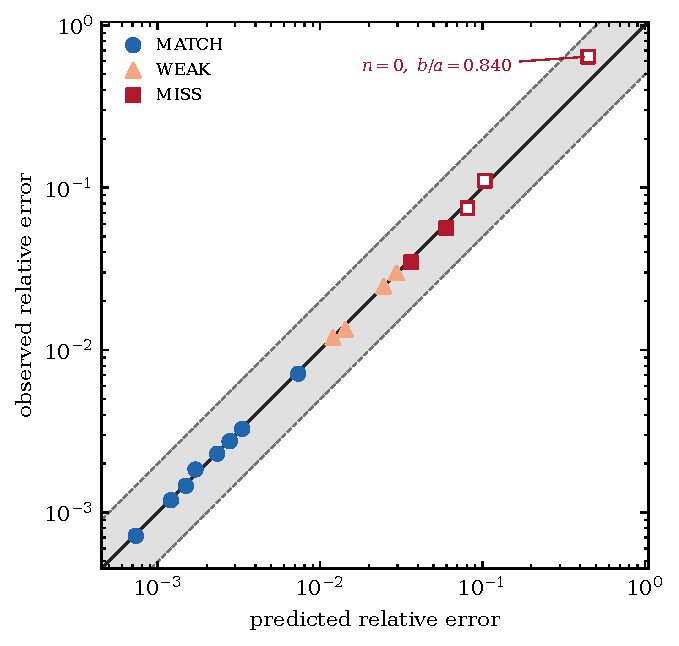
\includegraphics[width=0.78\linewidth]{southwell_pred_vs_obs}
\caption{Predicted versus observed relative miss on Southwell
Table~2.31, all eighteen rows, log--log. The solid line is identity;
the shaded band is a factor of two. Markers follow the same
MATCH/WEAK/MISS gate as the main-text table. Open squares are the three
rows whose stored forward value was a search-window endpoint; the
observed error plotted is from the wide re-search (daggers in
Table~\ref{tab:sm-inverse}). Ratio of predicted to observed error lies
between $0.70$ and $1.13$ on $18/18$.}
\label{fig:sm-predobs}
\end{figure}
\FloatBarrier

\subsection{Three rows were window endpoints}\label{sec:sm-inv-edge}
An audit of all $342$ stored rows in this study against each row's own search
window found twelve endpoint returns and no near-misses, all of them in the
mixed-edge sweep. Three of them are Southwell rows, and all three had been
counted as MISS, so correcting them does not change the $13/18$ score. It does
change the numbers, and the corrected values are what appear in the main text
and in Table~\ref{tab:sm-inverse}:

\begin{center}\small
\begin{tabular}{lccc}
\toprule
cell & printed $\lamsq$ & stored (endpoint) & re-searched $\lamsq$\\
\midrule
$n=0$, $\ba=0.840$ & 81.0 & --- & \textbf{132.990}\\
$n=3$, $\ba=0.71$  & 49.0 & --- & \textbf{45.346}\\
$n=3$, $\ba=0.82$  & 100  & --- & \textbf{111.041}\\
\bottomrule
\end{tabular}
\end{center}

\noindent
The stored endpoint values are deliberately not reproduced: an endpoint is a
property of the scanned window, not of the plate, and printing one beside a
frequency invites it to be read as one. In the two $n=3$ cases the true root
lies just \emph{outside} the half-window that was scanned, so the window was
too narrow rather than mis-centred. Correcting the three rows improves the
sensitivity result: the predicted-versus-observed ratio at $n=0$, $\ba=0.840$
falls from $3.13$ to $0.70$, which is what makes the unification $18/18$
rather than $17/18$.

The general lesson is recorded because it applies to any determinant search on
a fixed absolute window: the sign-flip ladder caught all twelve of these
(none classified CLEAN or FLOOR), but the MATCH/WEAK/MISS gate, being computed
from the relative miss alone, did not. One counted cell --- the $(1,1)$ entry
of Table~2.30 at $\ba=0.1$ --- was scored WEAK on an endpoint value, and its
re-searched root is also WEAK ($1.37\%$ at $\nu=0.30$, $1.56\%$ at
$\nu=1/3$), so the reported pass rate is unchanged. It was, however, right by
luck. Wiring the endpoint label into the scoring gate changes scoring and
would need its own pre-registration; it has deliberately not been done for
this paper.

\subsection{A secondary differential test, and why it is not
load-bearing}\label{sec:sm-inv-vogel}
A separate test asked whether Southwell's residual radius-ratio discrepancies
are larger than Vogel's when both are measured against the same model of
what rounding alone should produce, namely half a unit in the last printed
place of $\lamsq$ divided by the local slope. The bar was fixed in advance at
a ratio of three between the two medians, and the test passed: Vogel's median
ratio of observed to expected discrepancy was $1.70$, inside the calibration
band, against $7.25$ for Southwell.

It is nevertheless reported here as corroboration and not as evidence, for
three reasons that were visible only after the run. The Vogel distribution is
heavy-tailed --- its upper quartile is $8.00$ and $55$ of $151$ solved cells
exceed a ratio of three --- so the rounding model is an incomplete account of
the residual for \emph{both} tables, and comparing two medians drawn from
distributions this dispersed is weak. There is an uncontrolled radius-ratio
confound: Vogel's median ratio falls monotonically with $\ba$, from $9.70$ at
$\ba=0.1$ to about $1.1$ at $\ba=0.9$, while Southwell's worst rows sit at
large $\ba$ and the two tables sample different ranges, so a purely
$\ba$-dependent effect could reproduce the median difference with no
source-precision story at all. And the inverse probe reproduced the same
window-endpoint artifact in its own variable, returning one Vogel row at a
radius-ratio offset exactly equal to its own half-window. The test was a real
falsification opportunity that the sensitivity account could have failed and
did not; the finite-element result of the main text is what settles the
question.

\begin{thebibliography}{9}\small
\bibitem{mccune2026annular} G. McCune, D. Stutts, ``Exact wave-function
solution and spurious-mode discrimination for completely free annular sector
plates,'' companion paper, submitted (2026).
\bibitem{ansysSM} ANSYS, Inc., \emph{ANSYS Mechanical APDL}, Release 2025 R1,
ANSYS, Inc., Canonsburg, PA, USA (2025).
\end{thebibliography}
\end{document}
